% !Mode:: "TeX:UTF-8"
\documentclass[a4paper, 11pt]{article}
\usepackage{xeCJK}
\setCJKmainfont{AR PL UMing CN} 
\usepackage{comment} % enables the use of multi-line comments (\ifx \fi)
\usepackage{lipsum} %This package just generates Lorem Ipsum filler text.
\usepackage{fullpage} % changes the margin
\usepackage{hyperref}

\begin{document}
%Header-Make sure you update this information!!!!
\noindent

\large\textbf{Conclusion Report}
\hfill \textbf{Exchange Simulator Project / Team B} \\

\normalsize Course code: CS28011 \hfill Prof. Jian Cao \& Dr. James L. Mei\\

TA: Nengjun Zhu  \hfill Due Date: 2016/12/30 \\

Teammates:
%TODO all write your student number, check your name
Alexander Goscinski 116030990050

Ruth-Emely Pierau 116030990078

Valentin Rothoft
 %TODO valentin 

Yelinsheng(查汗巴依尔·叶林生) 116033910057

Husein Sulianto
 %TODO Husein



\section*{System Architecture}
\lipsum[2]

\section*{Key Techniques}

The project is mainly written in python. We used python 2.7. For some features like the matching algorithm the numpy library \cite{numpy} was used.
For the FIX communication we used the quickfix library. For the database we use MySQL and use the library MySQL-python as interface between python and MySQL.
\subsection*{Order Matching}

%TODO Valentin
\subsection*{FIX}
%TODO Husein
Talk about quickfix library

\subsection*{Database}

For the database MySQL 5.7.15 was used. We created the diagrams and sql scripts creating the structure of the database with MySQL Workbench.
As interface between python any MySQL we used MySQL-python version 1.2.5.
\subsubsection*{Server}
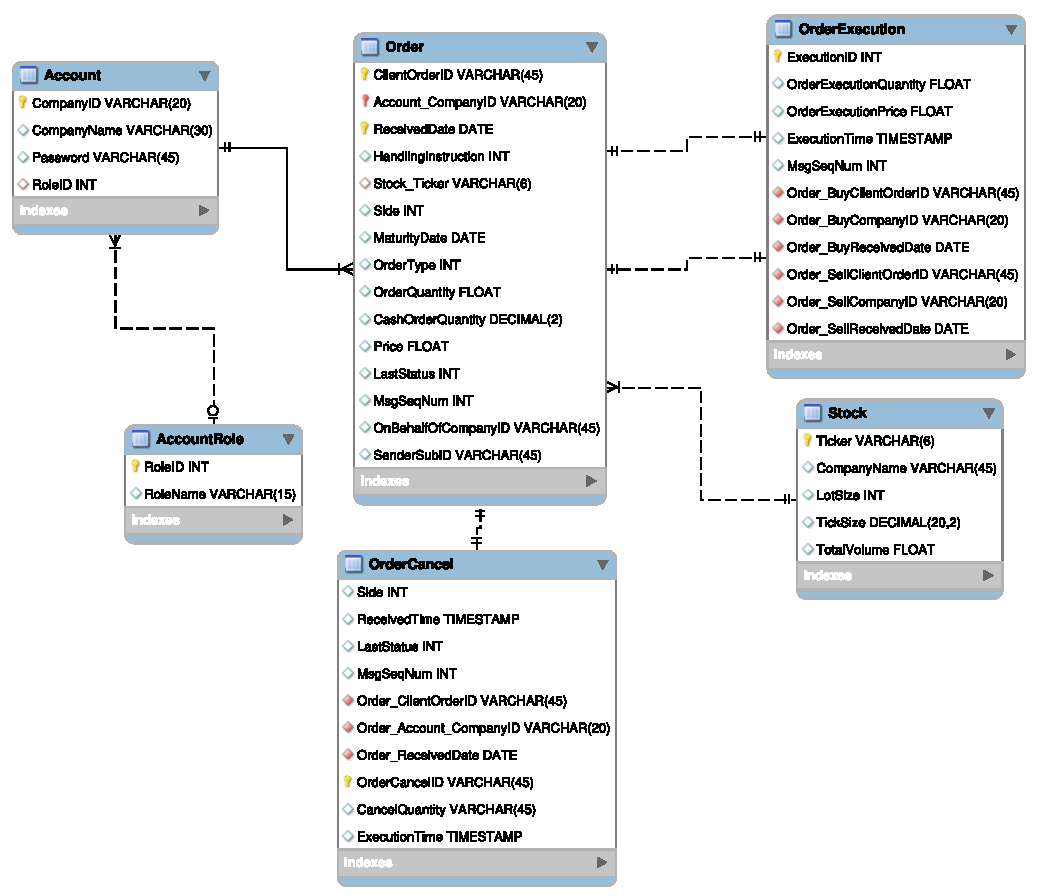
\includegraphics{../diagrams/server_database.pdf}
\paragraph*{Account}
A user account is used my clients to connect to the server

\textbf{CompanyID:} the ID of the company when the company registered
...
\subsubsection*{Client}
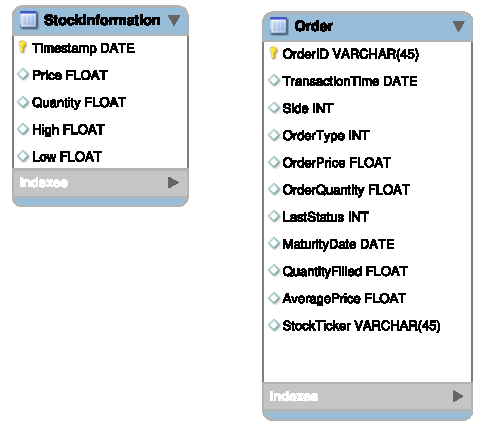
\includegraphics{../diagrams/client_database.pdf}
%TODO Husein

\subsection*{GUI}

\begin{itemize}
  \item Use python's GUI library HtmlPy to create GUI using html, css, javascript.
  \item Use CSS library Bootstrap to create fancy front end page. 
  \item Use JS library Jquery to add logic.
\end{itemize}




\section*{Task Allocation Among Members}

Alexander Goscinski:
\begin{itemize}
  \item Implementation and maintenance of system architecture
  \item Manage tasks
\end{itemize}
Ruth-Emely Pierau:
\begin{itemize}
	\item Implementation and testing of Matching Algorithm
	\item Implementation of some functions for testing server logic
	\item Implementation of some basic data classes
\end{itemize}
Yelinsheng(查汗巴依尔·叶林生):
\begin{itemize}
  \item GUI implementation
  \item Some functions of client logic
  \item Some functions of server logic
  \item Implementation of some basic data classes
  \item Code testing
\end{itemize}
Husein Sulianto:
\begin{itemize}
  \item Designing overview of Database
  \item Do Order Canceling function in client and server side
  \item Implementation of several basic data classes and fix message definition layout
  \item Code testing
\end{itemize}
Valentin
%TODO Valentin

% to comment sections out, use the command \ifx and \fi. Use this technique when writing your pre lab. For example, to comment something out I would do:
%  \ifx
%   \begin{itemize}
%       \item item1
%       \item item2
%   \end{itemize}
%  \fi

\section*{Workload Allocations}
Total 100\% \\

\section*{Other}
\lipsum[7]

\section*{Conclusion}
The usage of the quickfix library with pythos is recommended because the port is not fitted to python code. It is mostly Java code with python grabbers.

\section*{Attachments}
Project homepage with installation instructions: \url{https://github.com/agoscinski/fsc} \\
Demo video (password: sjtu1896): \url{https://owncloud.tu-berlin.de/index.php/s/ihEUWxj8FvIAZhI}

\begin{thebibliography}{9}
\bibitem{numpy} Developers, NumPy. "NumPy." NumPy Numpy. Scipy Developers (2013) \url{https://docs.scipy.org/doc/numpy-dev/numpy-ref.pdf}.
\end{thebibliography}

\end{document}
